\newpage
\section{結果}
\subsection{実習2-1 課題実験}
\begin{itemize}
\item プログラム\ref{ex21-block}は定電圧を100回測定するプログラムである.このようにNの数を99にすることで100回のデータ測定が可能となる.
\item 実行後,フロントパネルでは,\wfig{ex21-flont}のように表示された.
\item \wtab{GND}から\wtab{fiveV}にGND,3.3\,\rm{V},5\,\rm{V}それぞれに接続した際の出力電圧を示す.
また,\wtab{means}は計測データから算出された平均値・標準偏差である.算出方法は\weq{mean},\weq{nut},\weq{keisan-nut}の通りである\cite{7d69cf97-0c1f}.導出過程で利用したExcel関数\weq{SUM}, \weq{SQRT}はそれぞれ,$\sum_{A}^{B}$, $\sqrt{A}$に対応している.
\begin{align}
平均値\,\rm{V}&:=(SUM(X_{0}:X_{99}))/100 (=MEAN_{v})\label{eq:mean}\\
標準偏差 - 推定値\,\rm{V}&:=STDEV.S(X_{0}:X_{99})\label{eq:nut}\\
標準偏差 - 計算値\,\rm{V}&:=SQRT((X_{i}-MEAN_{v})^2/99)\label{eq:keisan-nut}\\
X_{i}&:データのi番目 \nonumber \\
MEAN_{v}&:上で計算した平均値をとる定数.GND, 3.3\,\rm{V}, 5\,\rm{V}の場合の計3種類\nonumber\\
SUM(A:B)&:AからBまでの和を返すExcel関数\label{eq:SUM}\\
STDEV.S(A:B)&:引数AからBをもとに,母集団の標準偏差の推定値を返すExcel関数\label{eq:STDEV.S}\\
SQRT(A)&:Aの平方根を返すExcel関数\label{eq:SQRT}
\end{align}
\end{itemize}

\begin{figure}[h]
\centering
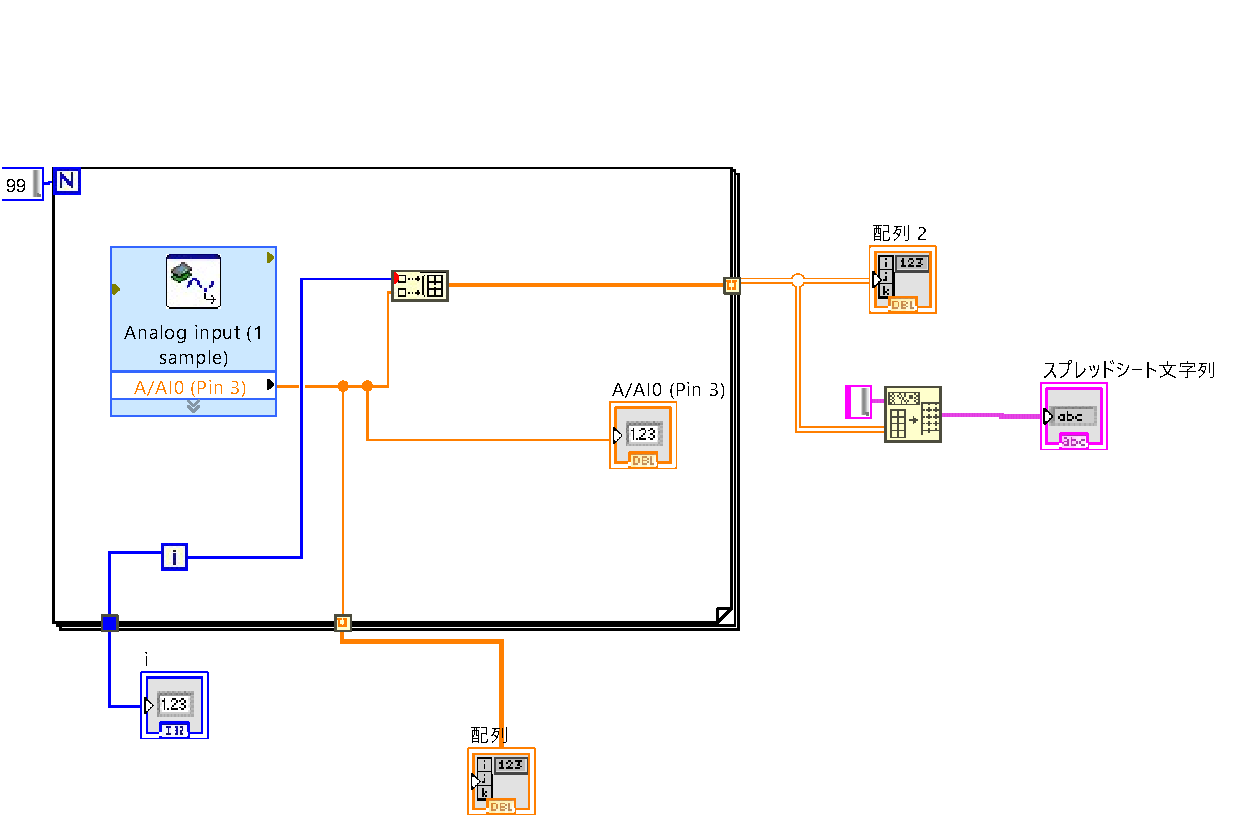
\includegraphics[scale=0.5]{./fig/ex21-block.pdf}\\
\useMycounter[\label{ex21-block}]定電圧計測のブロックダイアグラム
\end{figure}

\begin{table}[h]
\centering
\caption{Excelを用いて算出された平均値と標準偏差}
\label{tab:means}
\begin{tabular}{cccc}
\hline
    接続先 	\textbackslash 算出値 &平均値[\rm{V}] &標準偏差 - 推定値[\rm{V}]   & 標準偏差 - 計算値[\rm{V}]    \\
     \hline
  GND& 0.00636  & 0.000499  & 0.000499419 \\
3.3\,\rm{V} & 3.26256 & 0.000568 & 0.000567549 \\
 5\,\rm{V}& 4.998779 & 0.00000000000000981918 &  0.00000000000000981918 \\
\hline
\end{tabular}
\end{table}

\begin{figure}[h]
\centering
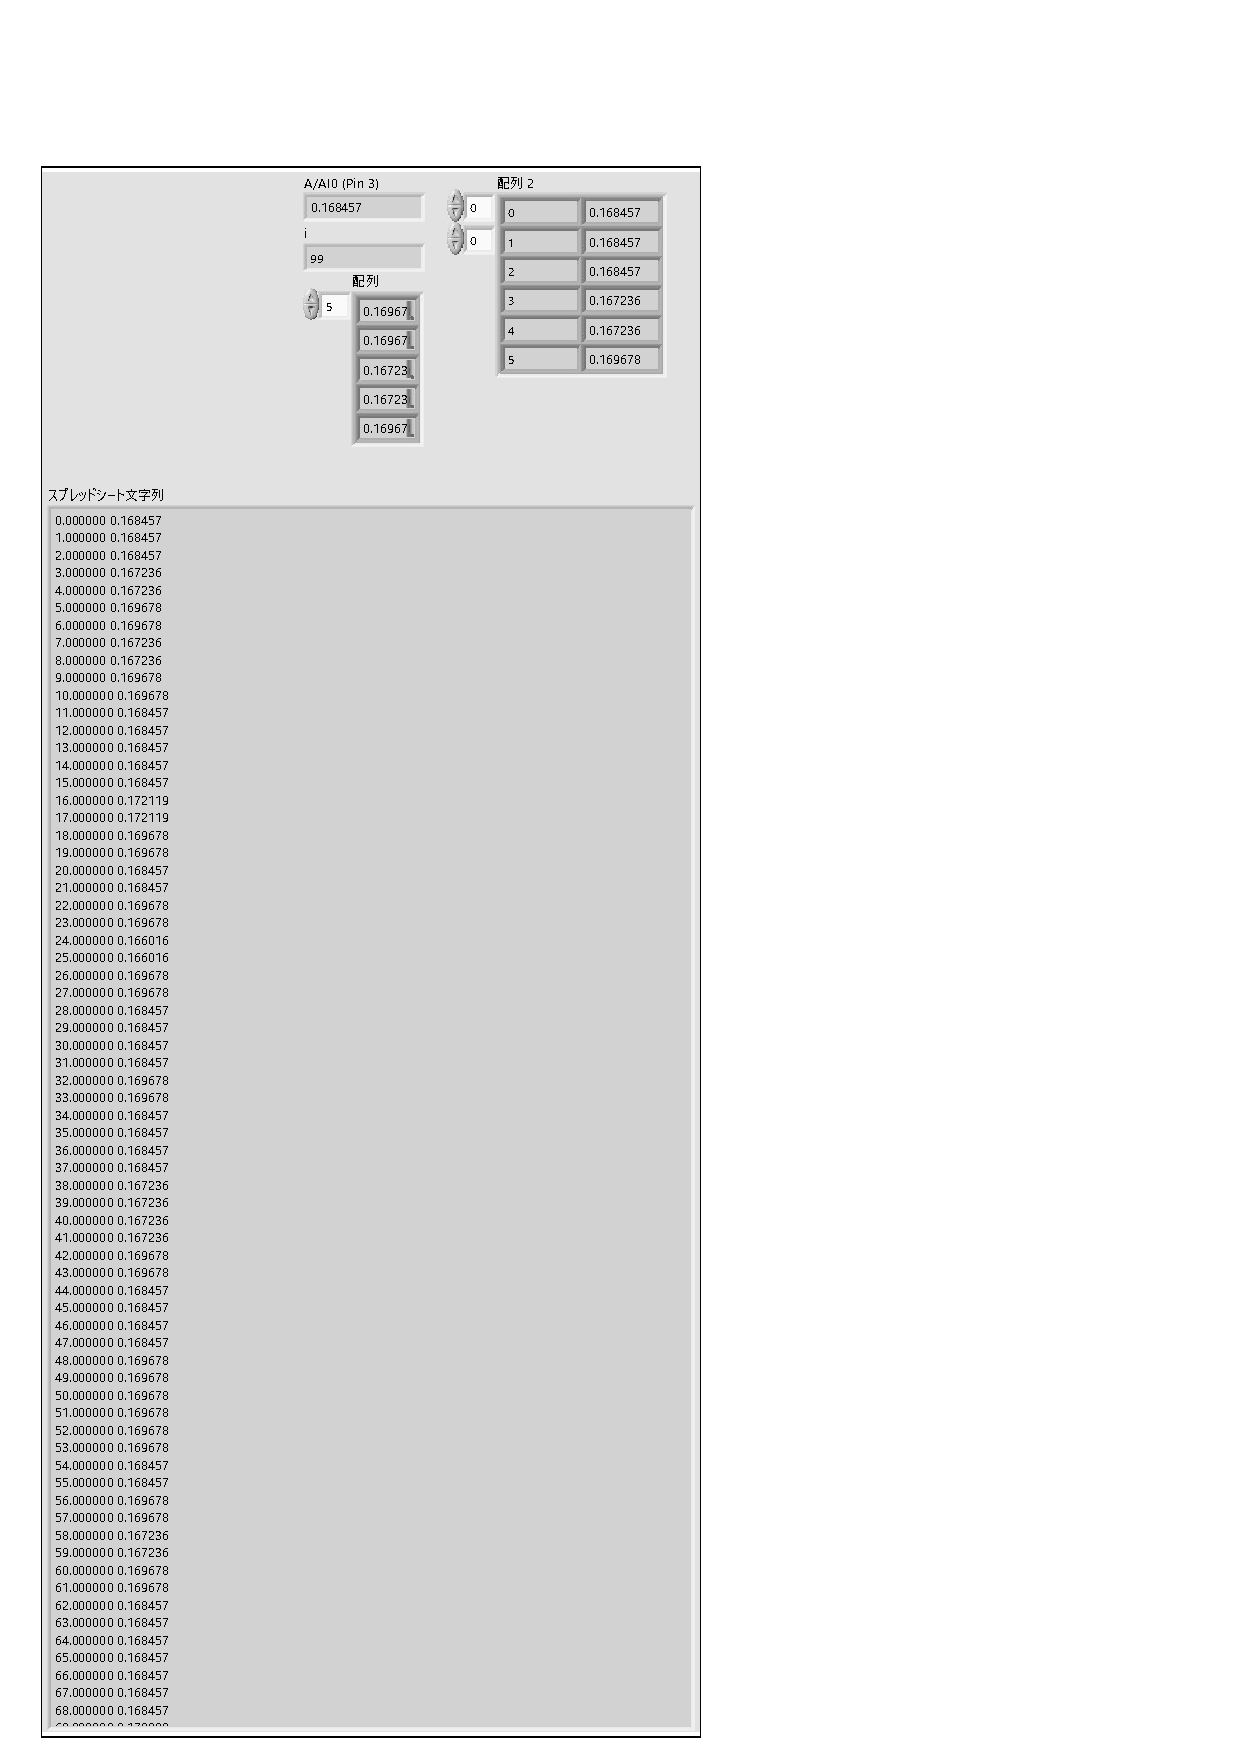
\includegraphics[scale=0.35]{./fig/ex21-flont.pdf}
\caption{定電圧計測のフロントパネル}
\label{fig:ex21-flont}
\end{figure}

\begin{table}[t]
\centering
 \caption{GND接続時の出力電圧}
 \label{tab:GND}
 \scalebox{0.7}{
\begin{tabular}{cccccccc}
\hline
測定回数[\rm{回}]&出力電圧[\rm{V}]&測定回数[\rm{回}]&出力電圧[\rm{V}]&測定回数[\rm{回}] &出力電圧[\rm{V}] &測定回数[\rm{回}] &出力電圧[\rm{V}] \\
\hline
0  & 0.006104 & 25 & 0.006104 & 50 & 0.006104 & 75 & 0.006104 \\
1  & 0.007324 & 26 & 0.007324 & 51 & 0.006104 & 76 & 0.006104 \\
2  & 0.006104 & 27 & 0.007324 & 52 & 0.006104 & 77 & 0.006104 \\
3  & 0.007324 & 28 & 0.007324 & 53 & 0.006104 & 78 & 0.006104 \\
4  & 0.007324 & 29 & 0.007324 & 54 & 0.006104 & 79 & 0.006104 \\
5  & 0.006104 & 30 & 0.007324 & 55 & 0.006104 & 80 & 0.006104 \\
6  & 0.006104 & 31 & 0.006104 & 56 & 0.006104 & 81 & 0.006104 \\
7  & 0.006104 & 32 & 0.006104 & 57 & 0.006104 & 82 & 0.007324 \\
8  & 0.006104 & 33 & 0.006104 & 58 & 0.006104 & 83 & 0.007324 \\
9  & 0.006104 & 34 & 0.006104 & 59 & 0.006104 & 84 & 0.006104 \\
10 & 0.006104 & 35 & 0.007324 & 60 & 0.006104 & 85 & 0.006104 \\
11 & 0.006104 & 36 & 0.007324 & 61 & 0.006104 & 86 & 0.007324 \\
12 & 0.006104 & 37 & 0.006104 & 62 & 0.006104 & 87 & 0.007324 \\
13 & 0.007324 & 38 & 0.006104 & 63 & 0.006104 & 88 & 0.006104 \\
14 & 0.007324 & 39 & 0.006104 & 64 & 0.006104 & 89 & 0.006104 \\
15 & 0.007324 & 40 & 0.006104 & 65 & 0.006104 & 90 & 0.006104 \\
16 & 0.006104 & 41 & 0.006104 & 66 & 0.006104 & 91 & 0.006104 \\
17 & 0.006104 & 42 & 0.006104 & 67 & 0.006104 & 92 & 0.006104 \\
18 & 0.006104 & 43 & 0.006104 & 68 & 0.006104 & 93 & 0.006104 \\
19 & 0.006104 & 44 & 0.006104 & 69 & 0.006104 & 94 & 0.006104 \\
20 & 0.006104 & 45 & 0.006104 & 70 & 0.006104 & 95 & 0.006104 \\
21 & 0.006104 & 46 & 0.006104 & 71 & 0.006104 & 96 & 0.006104 \\
22 & 0.007324 & 47 & 0.006104 & 72 & 0.006104 & 97 & 0.007324 \\
23 & 0.007324 & 48 & 0.006104 & 73 & 0.006104 & 98 & 0.007324 \\
24 & 0.006104 & 49 & 0.006104 & 74 & 0.006104 & 99 & 0.006104\\
\hline
\end{tabular}
}
 \end{table}
 
\begin{table}[b]
 \centering
 \caption{3.3\,\rm{V}接続時の出力電圧}
 \label{tab:three-threeV}
\scalebox{0.7}{
\begin{tabular}{cccccccc}
\hline
測定回数[\rm{回}]&出力電圧[\rm{V}]&測定回数[\rm{回}]&出力電圧[\rm{V}]&測定回数[\rm{回}] &出力電圧[\rm{V}] &測定回数[\rm{回}] &出力電圧[\rm{V}] \\
\hline
0  & 3.262939 & 25 & 3.262939 & 50 & 3.261718 & 75 & 3.262939 \\
1  & 3.262939 & 26 & 3.262939 & 51 & 3.262939 & 76 & 3.262939 \\
2  & 3.262939 & 27 & 3.262939 & 52 & 3.262939 & 77 & 3.262939 \\
3  & 3.262939 & 28 & 3.262939 & 53 & 3.262939 & 78 & 3.262939 \\
4  & 3.262939 & 29 & 3.262939 & 54 & 3.262939 & 79 & 3.261718 \\
5  & 3.261718 & 30 & 3.262939 & 55 & 3.262939 & 80 & 3.261718 \\
6  & 3.261718 & 31 & 3.262939 & 56 & 3.262939 & 81 & 3.262939 \\
7  & 3.262939 & 32 & 3.262939 & 57 & 3.262939 & 82 & 3.262939 \\
8  & 3.262939 & 33 & 3.262939 & 58 & 3.262939 & 83 & 3.262939 \\
9  & 3.262939 & 34 & 3.261718 & 59 & 3.262939 & 84 & 3.262939 \\
10 & 3.262939 & 35 & 3.261718 & 60 & 3.262939 & 85 & 3.261718 \\
11 & 3.262939 & 36 & 3.261718 & 61 & 3.262939 & 86 & 3.261718 \\
12 & 3.262939 & 37 & 3.261718 & 62 & 3.262939 & 87 & 3.262939 \\
13 & 3.261718 & 38 & 3.261718 & 63 & 3.262939 & 88 & 3.262939 \\
14 & 3.261718 & 39 & 3.261718 & 64 & 3.262939 & 89 & 3.262939 \\
15 & 3.261718 & 40 & 3.261718 & 65 & 3.262939 & 90 & 3.262939 \\
16 & 3.261718 & 41 & 3.262939 & 66 & 3.262939 & 91 & 3.262939 \\
17 & 3.262939 & 42 & 3.262939 & 67 & 3.262939 & 92 & 3.262939 \\
18 & 3.262939 & 43 & 3.261718 & 68 & 3.262939 & 93 & 3.262939 \\
19 & 3.262939 & 44 & 3.261718 & 69 & 3.262939 & 94 & 3.262939 \\
20 & 3.262939 & 45 & 3.261718 & 70 & 3.262939 & 95 & 3.262939 \\
21 & 3.262939 & 46 & 3.261718 & 71 & 3.261718 & 96 & 3.262939 \\
22 & 3.261718 & 47 & 3.262939 & 72 & 3.261718 & 97 & 3.262939 \\
23 & 3.261718 & 48 & 3.262939 & 73 & 3.261718 & 98 & 3.261718 \\
24 & 3.262939 & 49 & 3.261718 & 74 & 3.261718 & 99 & 3.261718 \\
\hline
\end{tabular}
}
\end{table}

\begin{table}[t]
\centering
 \caption{5\,\rm{V}接続時の出力電圧}
 \label{tab:fiveV}
 \scalebox{0.7}{
\begin{tabular}{cccccccc}
\hline
測定回数[\rm{回}]&出力電圧[\rm{V}]&測定回数[\rm{回}]&出力電圧[\rm{V}]&測定回数[\rm{回}]&出力電圧[\rm{V}]&測定回数[\rm{回}]&出力電圧[\rm{V}]\\
\hline
0  & 4.998779 & 25 & 4.998779 & 50 & 4.998779 & 75 & 4.998779 \\
1  & 4.998779 & 26 & 4.998779 & 51 & 4.998779 & 76 & 4.998779 \\
2  & 4.998779 & 27 & 4.998779 & 52 & 4.998779 & 77 & 4.998779 \\
3  & 4.998779 & 28 & 4.998779 & 53 & 4.998779 & 78 & 4.998779 \\
4  & 4.998779 & 29 & 4.998779 & 54 & 4.998779 & 79 & 4.998779 \\
5  & 4.998779 & 30 & 4.998779 & 55 & 4.998779 & 80 & 4.998779 \\
6  & 4.998779 & 31 & 4.998779 & 56 & 4.998779 & 81 & 4.998779 \\
7  & 4.998779 & 32 & 4.998779 & 57 & 4.998779 & 82 & 4.998779 \\
8  & 4.998779 & 33 & 4.998779 & 58 & 4.998779 & 83 & 4.998779 \\
9  & 4.998779 & 34 & 4.998779 & 59 & 4.998779 & 84 & 4.998779 \\
10 & 4.998779 & 35 & 4.998779 & 60 & 4.998779 & 85 & 4.998779 \\
11 & 4.998779 & 36 & 4.998779 & 61 & 4.998779 & 86 & 4.998779 \\
12 & 4.998779 & 37 & 4.998779 & 62 & 4.998779 & 87 & 4.998779 \\
13 & 4.998779 & 38 & 4.998779 & 63 & 4.998779 & 88 & 4.998779 \\
14 & 4.998779 & 39 & 4.998779 & 64 & 4.998779 & 89 & 4.998779 \\
15 & 4.998779 & 40 & 4.998779 & 65 & 4.998779 & 90 & 4.998779 \\
16 & 4.998779 & 41 & 4.998779 & 66 & 4.998779 & 91 & 4.998779 \\
17 & 4.998779 & 42 & 4.998779 & 67 & 4.998779 & 92 & 4.998779 \\
18 & 4.998779 & 43 & 4.998779 & 68 & 4.998779 & 93 & 4.998779 \\
19 & 4.998779 & 44 & 4.998779 & 69 & 4.998779 & 94 & 4.998779 \\
20 & 4.998779 & 45 & 4.998779 & 70 & 4.998779 & 95 & 4.998779 \\
21 & 4.998779 & 46 & 4.998779 & 71 & 4.998779 & 96 & 4.998779 \\
22 & 4.998779 & 47 & 4.998779 & 72 & 4.998779 & 97 & 4.998779 \\
23 & 4.998779 & 48 & 4.998779 & 73 & 4.998779 & 98 & 4.998779 \\
24 & 4.998779 & 49 & 4.998779 & 74 & 4.998779 & 99 & 4.998779\\
\hline
\end{tabular}
}
\end{table}
